\graphicspath{{roots_2ext/}}

\chapter[Computing in Degree $2^k$-Extensions of Finite Fields of \\ Odd Characteristic]
{Computing in Degree $2^k$-Extensions of Finite Fields of Odd Characteristic}
\label{chapter:2ext-op}

\section{Introduction}\label{section:intro}


Factoring polynomials and constructing irreducible polynomials are two
fundamental operations for finite field arithmetic. As of now, there
exists no deterministic polynomial time algorithm for these questions
in general, but in some cases better answers can be found. In this
chapter, we discuss algorithmic questions arising in such a special case:
the construction of, and computations with, extensions of degree
$n=2^k$ of a base field, say $\F_q$, with $q$ a power of an odd prime
$p$. In other words, we are interested with the complexity of
computing in the quadratic closure of $\F_q$.

There exists a well-known construction of such
extensions~\cite[Th.\ VI.9.1]{Lang02}, which was already put to use
algorithmically in~\cite{Shoup94}: if $q=1\bmod 4$, then for any
quadratic non-residue $\alpha \in \F_q$, the polynomial
$X^{2^k}-\alpha \in \F_q[X]$ is irreducible for any $k \ge 0$, and
allows us to construct $\F_{q^{2^k}}$. If $q=3\bmod 4$, we first
construct a degree-two extension $\F_{q'}$ of $\F_q$, which will thus
satisfy $q' = 1 \bmod 4$; this is done by remarking that $X^2+1 \in
\F_q[X]$ is irreducible, so that we can construct $\F_{q'}$ as
$\F_q[X]/\langle X^2+1 \rangle$.

In this note, taking this remark as a starting point, we give fast
algorithms for operations such as multiplication and inversion, trace
and norm computation, and most importantly square root computation in
$\F_{q^{2^k}}$ (see below for our motivation), as well as isomorphism
computation. 

We do not make any assumption on the way $\F_q$ is represented: the
running time of our algorithms is estimated by counting operations
$(+,\times,\div)$ in $\F_q$ at unit cost.  The cost of most algorithms
will be expressed in terms of the cost of polynomial
multiplication. Explicitly, we let $\MM:\N\to\N$ be such that degree
$n$ polynomials over any ring $R$ can be multiplied in $\MM(n)$
operations in $R$, and such that $\MM(n)/n$ is non-decreasing (this
will be referred to as {\em super-linearity}). Using the algorithm
of~\cite{CaKa91}, we can take $\MM(n)=O(n \log(n)\log\log(n))$.

In view of the discussion above, we will assume that $q = 1 \bmod 4$:
if this is not the case, replacing $\F_q$ by $\F_{q'}$ as explained
above only induces a constant overhead, since all operations
$(+,\times,\div)$ in $\F_{q'}$ can be done using $O(1)$ operations in
$\F_q$. Besides, we will assume that the non-quadratic residue
$\alpha$ is given; otherwise, such an $\alpha$ can be found by
testing an expected $O(1)$ random elements in $\F_q$ for quadratic
residuosity. This remains a core non-deterministic component of the
construction, since finding $\alpha$ in a polynomial-time
deterministic manner is a well-known open question. Some algorithms
below are non-deterministic (Las Vegas) as well; for such algorithms,
we give the expected running time.

\begin{theorem}\label{theo:main}
  Suppose that $q=1 \bmod 4$. Given a non-quadratic residue $\alpha
  \in \F_q$, for $k \ge 0$ and $n=2^k$, the running times for
  computations in $\F_{q^n}$ reported in Table~\ref{tab1} hold.
\end{theorem}

\begin{table}[h]
\begin{center}
\begin{tabular}{c|c}
Operation & Cost \\
\hline
addition / subtraction & $O(n)$\\
multiplication & $\MM(n)+O(n)$\\
inversion & $O(\MM(n))$\\
Frobenius & $O(n+\log(q))$\\
norm & $O(\MM(n))$ \\
trace & 1 \\ 
quadratic residuosity & $O(\MM(n)+\log(q))$ \\
square root &  $O(\MM(n)\log(nq))$\ \ (expected) \\
isomorphism &  $O(n + \log(n)\log(q))$\ \ (expected)
\end{tabular}
  \caption{Costs for computations in $\F_{q^n}$, with $n=2^k$.}
  \label{tab1}
\end{center}
\end{table}

This paper can be seen as an
analogue of~\cite{DeSc12}, which discusses these questions for
Artin-Schreier extensions: the problems we consider, the techniques we
use, and the applications (dealing with torsion points of some genus 1
or 2 Jacobians; see below) are similar. More precisely, the recursive 
techniques used here are similar to those in the reference in terms of 
exploiting the special structure of the tower and the defining polynomials.

For some questions, such as Frobenius or isomorphism computation, we
refer to the next section for a precise description of the operation
we perform; however, we mention that in all cases, we use a polynomial
basis representation for all computations. In all cases, the combined
size of input and output is $O(n)$ elements in $\F_q$, and using fast
multiplication, all running times reported here are quasi-linear\footnote{
An algorithm is quasi-linear time in $n$ if it has complexity $O(n\log^kn)$
for a constant $k$.} in $n$.

Some results in the above table are straightforward (such as addition
/ subtraction or trace computation) and some are well-known (such as
multiplication). Our focus in this note is actually on square root
computation, and to the best of our knowledge, this is the first time
that such results appear. 

The straightforward approaches to square root extraction, using for
instance Cipolla's or the Tonelli-Shanks
algorithms~\cite{Tonelli1891, Cipolla1903, Shanks1972} require a number
of multiplications in $\F_{q^n}$ proportional to $\log(q^n)$; the
cost is then $O(n \MM(n)\log(q))$ operations in $\F_q$, which is
at best quadratic in $n$. It is possible to compute square roots faster,
using fast algorithms for {\em modular composition}, which is the
operation that consists in computing $F(G) \bmod H$,  given some
univariate polynomials $F,G,H$. Let us denote by $\CC(n)$ the cost of
this operation, when $F,G,H$ have all degree at most $n$. Then, the
algorithms of~\cite{KaltofenShoup1997,DlsSch2011} compute square roots
in $\F_{q^n}$ using $O(\MM(n)\log(q) + \CC(n)\log(n))$ operations in
$\F_q$.

In our model, where operations in $\F_q$ are counted at unit cost, the
best known bound on $\CC(n)$ is $\CC(n)=O(\sqrt{n}\MM(n) +
n^{(\omega+1)/2})$, where $2 \le \omega \le 3$ is such that matrices
of size $m$ over $\F_q$ can be multiplied in $O(m^\omega)$ operations \cite{BrKu78}.
Thus, depending on $\omega$, and neglecting logarithmic factors, the
cost (with respect to $n$) of the corresponding square root algorithms
ranges between $O(n^{3/2})$ and $O(n^{2})$. We remark however that, in
a boolean model (on a RAM, using an explicit boolean representation of the
elements in $\F_q$, and counting boolean operations at unit cost),
Kedlaya and Umans gave in~\cite{KeUm11} an algorithm of cost
$n^{1+\varepsilon} \log(q)^{1+o(1)}$ for modular composition in
$\F_q$, for any $\varepsilon > 0$. In that model, algorithms such as
those in~\cite{KaltofenShoup1997,DlsSch2011} are thus close to linear time.

None of the algorithms mentioned above is dedicated to the specific
case we consider, where the extension degree $n$ is a power of two;
few references consider explicitly this particular 
case~\cite{FeNoMo03, FeNoMo05}. 

The algorithm of~\cite{FeNoMo03} gives a quadratic residuosity test
that uses $O(\log(n))$ Frobenius computations and multiplications in
$\F_{q^n}$, and $O(\log(q))$ multiplications in $\F_q$. This reference
does not specify how to represent the extensions of $\F_q$, and what
algorithms should be used for basic operations.  Using the algorithms
given below for arithmetic and Frobenius computations, the cost of
their quadratic residuosity test algorithm is $O((\MM(n) +
\log(q))\log(n))$ multiplications in $\F_q$; this is slightly slower
than our result.  The authors of \cite{FeNoMo03} also give algorithms
for quadratic residuosity and square root computation for degree
$2^k$-extensions in their later work \cite{FeNoMo05}. They removed the
computation overlap between quadratic residuosity test and square
root, but the algorithms still run in times quadratic in $n$ (the
quadratic residuosity test being the bottleneck).

\medskip

This work was inspired by computations with Jacobians of curves of
genus 2 over finite fields. Given a genus 2 curve $C$ defined over
$\F_p$, the algorithm of~\cite{GaSc12} computes the cardinality of the
Jacobian $J$ of $C$, following Schoof's elliptic curve point counting
algorithm~\cite{Schoof85}. This involves in particular the computation
of successive divisors of $2^k$-torsion in $J$, by means of successive
divisions by two in $J$. Such a division by two boils down to several
arithmetic operations, and four square root extractions; thus, the
divisors we are computing are defined over the quadratic closure of
$\F_p$, or of a small extension of $\F_p$.

In other words, for dealing with $2^k$-torsion, the algorithm
of~\cite{GaSc12} relies entirely on the operations above, arithmetic
operations and square root extraction. At the time of
writing~\cite{GaSc12}, the authors relied on a variant of the
Kaltofen-Shoup algorithm~\cite{KaltofenShoup1997} with running time
$O(\MM(n)\log(q) + \CC(n)\log(n))$, which was a severe bottleneck; our
new algorithms completely alleviate this issue.

\medskip

After proving Theorem~\ref{theo:main} in Section~\ref{sec:proof}, we
present in Section~\ref{sec:exp} some experiments that confirm that
the practical interest of our quasi-linear algorithms for the
point-counting problem above.

\paragraph{Acknowledgements.} The authors are supported by NSERC and
the Canada Research Chairs program. We wish to thank the reviewers for
their helpful remarks and suggestions.

%%%%%%%%%%%%%%%%%%%%%%%%%%%%%%%%%%%%%%%%%%%%%%%%%%
%%%%%%%%%%%%%%%%%%%%%%%%%%%%%%%%%%%%%%%%%%%%%%%%%%

\section{Proof of the complexity statements}\label{sec:proof}

In this section, we prove the results stated in Table~\ref{tab1}.
The tower of fields $\F_q,\F_{q^2},\dots\F_{q^{2^k}},\dots$ will be
written
$$\L_0 \subset \L_1 \subset \cdots \subset \L_k \subset \cdots,$$ with
$\L_k = \F_{q^{2^k}}$ for all $k$.

%=================================================

\subsection{Representing the fields $\L_k$}

The tower of fields $\L_0,\L_1,\dots$ can be represented in two
fashions, using univariate or multivariate representations (see as
well~\cite{DeSc12}, for a similar discussion for Artin-Schreier
extensions).

Let $\alpha\in\F_q$ be a fixed non-quadratic residue.  Define the
sequence of polynomials $T_1,T_2,\dots$ in indeterminates
$X_1,X_2,\dots$ given by
$$T_1 = X_1^2-\alpha \quad\text{and}\quad T_k = X_k^2-X_{k-1}
\quad\text{for $k > 1$},$$ as well as the polynomials $P_1,P_2,\dots$ given by
$$P_k = X_k^{2^k} - \alpha\quad\text{for $k \ge 1$}.$$The discussion
in the introduction, as well as the one in~\cite{Lang02}, shows that for 
all $k \ge 0$ we have the equality between ideals
\begin{equation}\label{eq:TP}
\langle T_1,\dots,T_k \rangle = \langle P_k, X_{k-1}-X_k^2, \dots,
X_1-X_k^{2^{k-1}} \rangle,
\end{equation}
that this ideal (call it $A_k$) is prime, and that we have
$$\L_k \simeq \F_q[X_1,\dots,X_k]/ A_k.$$ 
For $k \ge 1$, let $x_k$ be the image of $X_k$ in the residue class
ring $\F_q[X_1,\dots,X_k]/A_k$.  Due to the natural embedding of
$\F_q[X_1,\dots,X_k]/ A_k$ into $\F_q[X_1,\dots,X_{k+1}]/ A_{k+1}$,
$x_k$ can be unequivocally seen as an element of $\F_{q^{2^\ell}}$ for $\ell
\ge k$ (and thus as an element of the quadratic closure of $\F_q$).

On the left-hand side of~\eqref{eq:TP}, we have a Gr{\"o}bner basis of
$A_k$ for the lexicographic order $X_1 < \cdots < X_k$, whereas on the
right we have a Gr{\"o}bner basis for the lexicographic order $X_k <
\cdots < X_1$. Corresponding to these two bases of $A_k$, the elements
of $\L_k$ can be represented as polynomials in $x_1,\dots,x_k$ of
degree at most $1$ in each variable (and coefficients in $\F_q$), or
as polynomials in $x_k$ of degree less than $2^k$.

By default, we will use the univariate representation; an element
$\gamma$ of $\L_k$ will thus be written as $\gamma=G(x_k)$, for some
polynomial $G \in \F_q[X_k]$ of degree less than $2^k$.

We will not explicitly need to convert to multivariate polynomials,
but we will often do one step of such a conversion, switching between
univariate and bivariate bases. Indeed, for all $k \ge 1$, we have
$$\L_k \simeq \F_q[X_k]/\langle P_k(X_k) \rangle \simeq \F_q[X_{k-1},X_k]/\langle
P_{k-1}(X_{k-1}), X_k^2-X_{k-1}\rangle.$$ The $\F_q$-monomial basis of
$\F_{q^{2^k}}$ associated to the left-hand side is
$$1,\ x_k,\ \dots,\ x_k^{2^k-1},$$ whereas the one associated to the
right-hand side is
$$1,\ x_{k-1},\ \dots,\ x_{k-1}^{2^{k-1}-1},\ x_k,\ x_{k-1}x_k,\ \dots,\ x_{k-1}^{2^{k-1}-1}x_k.$$
The change-of-basis from the univariate basis to the bivariate one
amounts to writing an expression $G(x_k)$, with $G$ of degree less
than $2^{k}$, as
$$G(x_k) = G_0(x_k^2) + x_k G_1(x_k^2) = G_0(x_{k-1}) + x_k
G_1(x_{k-1}),$$ with $G_0$ and $G_1$ of degrees less than
$2^{k-1}$. This does not require any arithmetic operation; the same
holds for the converse change-of-basis. Continuing this way on $G_0$
and $G_1$, we could convert between univariate and multivariate bases
without arithmetic operations if needed.

%=================================================

\subsection{Arithmetic operations}

In this subsection, we discuss the cost of arithmetic operations
$(+,\times,\div)$ in $\L_k$, for some $k \ge 0$.  In all that follows,
we write $n=[\L_k:\F_q]$, that is, $n=2^k$.

Addition and subtraction take time $O(n)$. For multiplication, using
the univariate basis leads to a cost of $\MM(n)+O(n)$ operations in
$\F_q$, where the $O(n)$ term accounts for reduction modulo $P_k$
(this takes linear time, since $P_k$ is a binomial). Note that a
non-trivial (and slightly less efficient) approach using the
multivariate representation is in~\cite{BoChHoSc11}.

For inversion, in the univariate basis, a natural idea is to use the
fast extended GCD algorithm for univariate
polynomials~\cite[Ch.~11]{GaGe03}, resulting in a running time
$O(\MM(n)\log(n))$. However, better can be done by using the tower
structure of the fields $\L_k$.  Indeed, consider $\gamma=G(x_k) \in
\L_k^\times$. Then, writing $G(x_k) = G_0(x_{k-1}) + x_k
G_1(x_{k-1}),$ we have
\begin{align*}
\frac{1}{G(x_k)}
&= \frac{1}{G_0(x_{k - 1}) + x_kG_1(x_{k - 1})}\\ 
&= \frac{G_0(x_{k-1}) - x_kG_1(x_{k-1})}{G_0(x_{k - 1})^2 - x_{k - 1}G_1(x_{k - 1})^2}.
\end{align*}
Therefore, computing an inverse in $\L_k$ amounts to $O(1)$ additions
and multiplications in $\L_k$, and one inversion in $\L_{k-1}$. This
gives a recursive algorithm with cost $T(k) = T(k-1) + O(\MM(2^k))$;
the super-linearity of $\MM$ implies that the running time is
$O(\MM(2^k))=O(\MM(n))$ operations in $\F_q$.

%=================================================

\subsection{Frobenius computation}

Let $\gamma$ be in $\L_k$, and let $r = q^d$ for some positive integer
$d$. We explain here how to compute $\gamma^r \in \L_k$; as above,
we write $n=2^k$.

We start with the case $\gamma=x_k$: writing $r = n u + v$ with $0 \le
v < n$, and using the fact that $x_k^n=\alpha$, we obtain $x_k^r =
\alpha^u x_k^v$. The constant $\alpha^u = \alpha^{u \bmod (q-1)}$ can
be computed in $O(\log(q))$ multiplications in $\F_q$ by repeated
squaring.  Although our focus is on counting $\F_q$-operations, we
also mention how to compute $u \bmod (q-1)$ and $v$ efficiently: first
of all, we compute $\rho=r\bmod n(q-1)$ by repeated squaring; then, $u
\bmod (q-1)$ and $v$ are respectively the quotient and remainder in
the division of $\rho$ by $n$. They can be computed with a boolean
cost polynomial (and actually, quasi-linear) in $\log(d)\log(nq)$,
since the bottleneck is an exponentation with exponent $O(d \log(q))$,
modulo an integer of bit size $O(\log(nq))$.

For a general $\gamma$ of the form $\gamma=G(x_k)$, 
writing $G(x_k) = g_{n - 1}x_k^{n - 1} + \cdots + g_1x_k + g_0$, we have
\begin{align*}
\gamma^r 
&= g_{n - 1}(x_k^r)^{n - 1} + \cdots + g_1(x_k^r) + g_0 \\
&= g_{n - 1}(\alpha^u x_k^v)^{n - 1} + \cdots + g_1(\alpha^u x_k^v) + g_0.
\end{align*}
Knowing $\alpha^u$ and $v$, computing $\gamma^r$ amounts to compute
the first $n$ powers of $\alpha^u x_k^v$ and substituting them in
$G$. Since $x_k^{n}=\alpha$, these powers are all monomials in $x_k$,
and can be computed successively in $O(n)$ multiplications in
$\F_q$. Therefore, computing the Frobenius takes a total of
$O(n+\log(q))$ operations in $\F_q$.

%=================================================

\subsection{Trace, norm and quadratic residuosity test}

The norm $\norm_{\L_k/\F_q}$ and the trace $\trace_{\L_k/\F_q}$
are easy to compute, using transitivity. Indeed, for $\gamma \in
\L_k$, we have
$$\norm_{\L_k / \F_q}(\gamma) = \norm_{\L_1 / \F_q}(\norm_{\L_2 / \L_1}(\cdots \norm_{\L_k / \L_{k -
    1}}(\gamma)))$$
and
$$\trace_{\L_k / \F_q}(\gamma) = \trace_{\L_1 / \F_q}(\trace_{\L_2 /
  \L_1}(\cdots \trace_{\L_k / \L_{k - 1}}(\gamma))).$$ Write as before
$\gamma=G(x_k)$ and $G=G_0(x_{k-1})+x_k G_1(x_{k-1})$.  Then, we have
$$\norm_{\L_k / \L_{k - 1}}(\gamma) =  G_0(x_{k - 1})^2 - x_{k - 1}G_1(x_{k - 1})^2$$
and
$$\trace_{\L_k / \L_{k - 1}}(\gamma) = 2G_0(x_{k - 1}),$$ since in the
quadratic extension $\L_k$ of $\L_{k-1}$ generated by $x_k^2-x_{k-1}$,
the norm (resp.\ trace) of $\gamma$ is the product (resp.\ sum) of
$\gamma$ and its conjugate $\gamma'=G_0(x_{k-1})-x_k G_1(x_{k-1})$.

To compute the norm of $\gamma$, this gives a recursive algorithm
using one recursive call and $O(1)$ multiplications in each extension;
using the super-linearity of $\MM$ (as for inversion), the total is
$O(\MM(n))$ operations in $\F_q$. For the trace, by transitivity, we
obtain $\trace_{\L_k / \F_q}(\gamma) = n g_0$ where $g_0$ is the constant
term of $G$; this could also have been deduced from the fact that the
trace of $\gamma=G(x_k)$ in the extension $\L_k=\F_q[X_k]/\langle P_k
\rangle$ is the coefficient of $X_k^{n-1}$ in $G P'_k \bmod P_k$.  At
any rate, the trace is computed using $1$ multiplication in $\F_q$

Finally, to check if $\gamma$ is a quadratic residue we compute
$\gamma^{(q^n - 1) / 2} = \norm_{\L_k / \F_q}(\gamma)^{(q - 1) / 2}$; this
takes $O(\MM(n) + \log(q))$ operations in $\F_q$ (using repeated squaring
for the exponentiation).

Let us briefly comment on alternative derivations of the norm and the
trace; they are slightly less efficient, but these ideas will allow us
to compute square roots in the next subsection (the underlying idea is
not new; it appears for instance in~\cite{GaSh92,FeNoMo03}).
Fix $n$ and $\gamma$ as above and for $m \ge 0$, define
$$N_m(\gamma) = \gamma^{1 + q + q^2 + \cdots + q^{m - 1}}$$ to be the
{\em $m$-norm} of $\gamma$. Similarly, the {\em $m$-trace} of $\gamma$
is defined to be $T_m(\gamma) = \gamma + \gamma^q + \cdots +
\gamma^{q^{m - 1}}$ (this is called a pseudo-trace
in~\cite{DeSc12}). For $m=n$, we recover the standard norm and trace.

Writing
$$\zeta_m = \gamma^{q + q^2 + \cdots + q^m},$$ we have $N_m(\gamma) = \gamma\zeta_{m
  - 1}$. The element $\zeta_m$ can be computed efficiently by means
of the formulas
\begin{equation}
\label{eq:zeta}
\zeta_1 = \gamma^q \quad\text{and}\quad
\zeta_m = 
\begin{cases}
\zeta_{m / 2}\zeta_{m / 2}^{q^{m / 2}} & \text{if $m$ is even}  \\
\zeta_1\zeta_{m - 1}^{q} & \text{if $m$ is odd.}
\end{cases} 
\end{equation}
(We could compute $N_m(\gamma)$ directly using a similar recurrence,
but we will reuse the $\zeta_m$ in the next subsection.)  Computing
$\zeta_1$ is done by means of one Frobenius computation.  Deducing
$\zeta_m$ from either $\zeta_{m / 2}$ or $\zeta_{(m-1) / 2}$ takes
$O(1)$ Frobenius and multiplications. Thus, the total for $\zeta_m$,
and thus $N_m(\gamma)$, is $O(\log(m))$ Frobenius and multiplications
in $\L_k$, which amounts to $O(\MM(n)\log(m)+\log(q)\log(m))$
operations in $\F_q$.

If needed, the $m$-trace can be computed similarly to the $m$-norm by
the following recursion:
$$T_1 = \gamma \quad\text{and}\quad
T_m = 
\begin{cases}
T_{m / 2} + T_{m / 2}^{q^{m / 2}} & \text{if $m$ is even}  \\
T_1 + T_{m - 1}^{q} & \text{if $m$ is odd.}
\end{cases}
$$ Therefore, $T_m(\gamma)$ can be computed using $O(\log(m))$
Frobenius and additions, hence the overall running time
$O(n\log(m)+\log(q)\log(m))$.


%=================================================

\subsection{Taking square roots}\label{section:sqrt}

In this subsection, we review the idea presented in \cite{DlsSch2011}
to compute square roots, and adapt it to our situation, where
computing a Frobenius is cheap.


Let $\delta \in \L_k^\times$ be given, assume that $\delta$ is a
square and let $\gamma \in \L_k$ be an (unknown) square root of
it. Define $\beta \in \F_q$ as the (unknown) quantity
\begin{equation}
\label{equation:tr-square}
\begin{aligned}
\beta = \trace_{\L_k / \F_q}(\gamma) = \sum_{i = 0}^{n - 1} \gamma^{q^i}
& = \gamma(1 + \gamma^{q - 1} + \gamma^{q^2 - 1} + \cdots + \gamma^{q^{n - 1} -1}) \\
& = \gamma(1 + \delta^{(q - 1) / 2} + \delta^{(q^2 - 1) / 2} + \cdots + \delta^{(q^{n - 1} -1) / 2})\\
& = \gamma \eta,
\end{aligned}
\end{equation}
with
$$\eta = 1 + \delta^{(q - 1) / 2} + \delta^{(q^2 - 1) / 2} + \cdots +
\delta^{(q^{n - 1} -1) / 2}.$$ We may assume $\eta \ne 0$; otherwise,
we can replace $\delta$ by $\delta' = \delta c^2$ for a random element
$c \in \L_k^\times$. We expect to have $\trace_{\F_q / \F_{q'}}(\gamma c) \ne 0$ 
after $O(1)$ trials: There are $q^{2^k} / q$ values of $c$ for which the trace is zero, 
and hence the probability of having a non-zero trace is $1 - (q^{2^k} / q) / q^{2^k} = 1 - 1/q
\ge 1/2$. Squaring both sides of Eq.~\eqref{equation:tr-square}
results in the quadratic equation $\beta^2 = \delta \eta^2$ over
$\F_q$.

Provided $\eta$ is known, $\beta$ can be deduced from this quadratic
equation, and finally $\gamma$ as $\gamma=\beta \eta^{-1}$.  Computing
$\beta$ from the above quadratic equation takes an expected
$O(\log(q))$ operations in $\F_q$~\cite[Ch.\ 14.5]{GaGe03}, so that
computing $\eta$ is the key to computing $\gamma$ efficiently. This
can be done as follows.

Let $\lambda \in \L_k$ be defined by $\lambda = \delta^{(q - 1) /
  2}$; then, $\eta$ is given by
$$
\eta = 1 + \lambda + \lambda^{1 + q} + \lambda^{1 + q + q^2} + \cdots + \lambda^{1 + q + q^2 + \cdots + q^{n-2}}.
$$
For $m \ge 0$, define 
$$\varepsilon_m = \lambda^{q} + \lambda^{q + q^2} + \cdots +
\lambda^{q + q^2 + \cdots + q^m},$$ so that $\eta= 1 + \lambda+
\lambda \varepsilon_{n-2}$, and recall as well the definition of
$\zeta_m = \lambda^{q + q^2 + \cdots + q^m}.$ Then, similar to the
recurrence relation given in~\eqref{eq:zeta} for $\zeta$, the following
holds for $\varepsilon$:
\begin{equation}\label{eq:varepsilon}
\varepsilon_1 =
\lambda^q \quad\text{and}\quad 
\varepsilon_m = 
\begin{cases}
\varepsilon_{m / 2} + \zeta_{m / 2}\varepsilon_{m / 2}^{q^{m / 2}} & \text{if $m$ is even}  \\
\varepsilon_{m-1} + \zeta_m & \text{if $m$ is odd}
\end{cases}  
\end{equation}
Computing $\lambda$ takes $O(\MM(n)\log(q))$ operations in $\F_q$;
then, we obtain the initial values $\zeta_1$ and $\varepsilon_1$ using
$O(1)$ Frobenius. Assume, inductively, that we have computed
$\varepsilon_m$, $\zeta_m$. Then, using Eqs.~\eqref{eq:zeta}
and~\eqref{eq:varepsilon}, $\zeta_{2m}$ and $\varepsilon_{2m}$, or
$\zeta_{2m+1}$ and $\varepsilon_{2m+1}$, can be computed using $O(1)$
Frobenius and $O(1)$ multiplications in $\F_{q^n}$. Therefore,
$\varepsilon_n$, and altogether $\eta =
1+\lambda+\lambda\varepsilon_{n-2}$ can be computed using
$O(\MM(n)\log(q)+\MM(n)\log(n))=O(\MM(n)\log(nq))$ operations in $\F_q$.
We have seen that deducing $\beta$ takes an expected $O(\log(q))$
operations in $\F_q$, and the cost of computing $\gamma$ is negligible
compared to the computation of $\eta$. Thus, the overall running time
is an expected $O(\MM(n)\log(nq))$ operations in $\F_q$.

%=================================================

\subsection{Computing embeddings}

We finally consider the problem of computing embeddings and
isomorphisms between two different ``towers'' defining the quadratic
closure of $\F_q$.  Consider $\L_k = \F_q[X_k]/\langle P_k \rangle$
and $\L'_j = \F_q[Y_j]/\langle Q_j\rangle$,  $k, j$ positive
integers, where we write
$$P_k = X_k^{2^k} - \alpha\quad\text{and}\quad Q_j = Y_j^{2^j} -
\beta,$$ for some non-quadratic residues $\alpha,\beta$ in $\F_q$.
Assuming for instance that $k \le j$, $\L_k$ can be identified as a
subfield of $\L'_j$; we show how to compute an embedding $\phi : \L_k
\hookrightarrow \L'_j$ efficiently. As before, we denote by $x_k$ the
image of $X_k$ in $\L_k$, and by $y_j$ the image of $Y_j$ in $\L'_j$;
we write $n=2^k$ and $m=2^j$.

The idea is straightforward: we first find a root $\rho$ of $P_k$ in
$\L'_j$; then, the mapping $\phi: \L_k \to \L'_j$ given by
$\phi(G(x_k)) = G(\rho) \bmod Q_j$ is well-defined and gives an
isomorphism of $\L_k$ onto its image. To find the root $\rho$ of
$P_k$ in $\L'_j$, one has to take $k$ successive square roots of
$\alpha$ in $\L'_j$. For this, we could use the algorithm of the
previous subsection, but since we start from $\alpha \in \F_q$, better
can be done.

Let us look at a slightly more general question: given $\mu \in \F_q$
and an even integer $\ell \ge 0$, compute a square root of $\mu
y_j^\ell$:
\begin{itemize}
\item if $\mu$ is a square in $\F_q$, say $\mu=\nu^2$, $\nu
  y_j^{\ell/2}$ is a square root of $\mu y_j^\ell$;
\item else, $\mu/\beta$ is a square in $\F_q$, say $\mu/\beta =
  \nu^2$; then $\nu y_j^{2^{j-1}+\ell/2}$ is a square root
  of $\mu y_j^\ell$.
\end{itemize}
Since we start with $\ell=0$, we can repeat the process at least $j$
times, and thus in particular at least $k$ times; the cost is thus
that of $O(k)=O(\log(n))$ quadratic residuosity tests, square-root
computations and arithmetic operations in $\F_q$; this uses an
expected $O(\log(q)\log(n))$ operations in $\F_q$.
Since the root $\rho$ we obtain is of the form $\rho=\mu
y_j^\ell$ for some $\ell < m$, computing $G(\rho) \mod Q_j$, for some
$G$ of degree less than $n$ (and thus than $m$), takes $O(m)$
multiplications in $\F_q$ (as was the case for Frobenius computation).

For isomorphism computation, taking $k=j$, and thus $m=n$, gives
the claimed bound $O(n + \log(q)\log(n))$ operations in $\F_q$.

%%%%%%%%%%%%%%%%%%%%%%%%%%%%%%%%%%%%%%%%%%%%%%%%%%
%%%%%%%%%%%%%%%%%%%%%%%%%%%%%%%%%%%%%%%%%%%%%%%%%%

\section{Experiments}\label{sec:exp}

We conclude this section with experiments using an implementation of
our algorithms based on NTL~\cite{NTL2009}. All running times are
obtained on an Intel Xeon CPU. In all cases, we start from the base
field $\F_p$.

First, we consider square root computation. For computing square roots
in an extension $\F_{p^n}$, without assumption on $n$, we used
in~\cite{DlsSch2011} modular polynomial composition, resulting in the
running time $O(\MM(n)\log(p) + \CC(n)\log(n))$. In cases where $n$ is
a power of two, the results in this paper are superior in terms of
complexity; Figure~\ref{figure:sqrtTiming} confirms that this is also
the case in practice. In that figure, we take the ``random'' prime $p
= \seqsplit{348975609381470925634534573457497}$ already used
in~\cite{DlsSch2011}, and different values of the extension degree~$n$,
that are always powers of two; see below for the reasons behind our
choice of such a large value of $p$.

\begin{figure}[ht]
\begin{center}
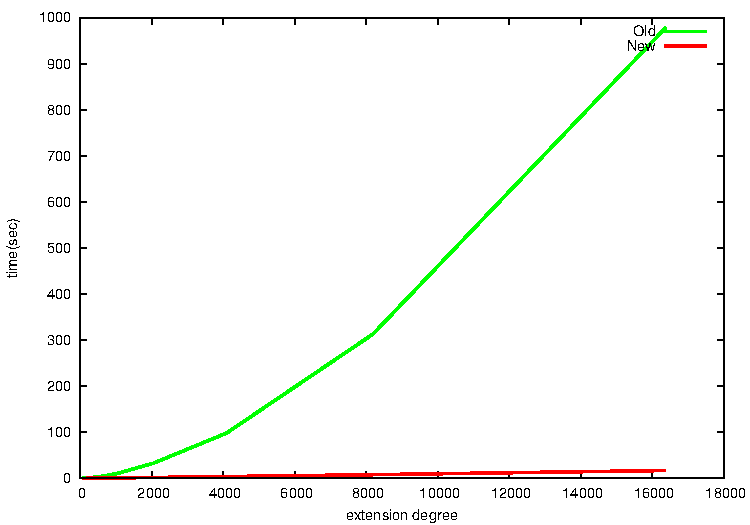
\includegraphics[width = 9cm]{sqrtTiming.pdf}
\end{center}
\caption{\small The new square root algorithm vs. the one in \cite{DlsSch2011}}
\label{figure:sqrtTiming}
\end{figure}

Table~\ref{table:2-tor-timings} gives timings (in seconds) for the
genus 2 point-counting application described in the introduction.  The
table describes the various ingredients involved in computing
successive $2^k$-torsion divisors in the Jacobian of the (randomly
chosen) curve $C$:
\[
\begin{array}{rcl}
y^2 &=& 
x^5 + 67412365472663169119085380769732137727\, x^4 \\
&& + 132706051439871719391705031627238584248\, x^3 \\
&& + 150906984006321211274278480789580538770\, x^2 \\
&& + 5602222826077482782805347307759926224\, x \\
&& + 157456212652423046465778673243920804193.
\end{array}
\]
over $\vmathbb{F}_p$ with $p = 2^{127} - 1$ (this 127 bit prime is the
one used in the records described in~\cite{GaSc12}). Once these
divisors are known, they are used to compute the cardinality of the
Jacobian $J$ of $C$ modulo $2^k$ (more exactly, we compute the image
modulo $2^k$ of the characteristic polynomial of the Frobenius
endomorphism on $J$); this last step is not detailed here, we will
refer to it as the {\em search} step.

In Table~\ref{table:2-tor-timings}, the degree $e_k$ is the degree of
the field extension over which the successive divisors are
defined. There are two main rows: the first one gives the timings for
computing all required square roots (which give us the required
$2^k$-torsion divisors); the second row gives the timing for the
search step, which involves arithmetic operations in the current
extension of $\F_p$. For a more precise profiling, each of the two
main rows is divided into three subrows labelled with \Romnum{1},
\Romnum{2}, and \Romnum{3}: \Romnum{1} denotes the original Gaudry and
Schost implementation~\cite{GaSc12}; \Romnum{2} and \Romnum{3} denote
the same implementation but using the algorithm in \cite{DlsSch2011}
and the one in Section \ref{section:sqrt} respectively. All square root
algorithms in this table are probabilistic.

In previous implementations, square root computation was a clear
bottleneck; with our new algorithm, it has now become a minor
component of the running time.



\begin{center}
\renewcommand{\multirowsetup}{\centering}
\renewcommand{\tabcolsep}{1.7mm}
% preventing the expont to touch the top of the cell
\newlength{\lengthofcell}
\newcommand{\pboxc}[1]{
\settowidth{\lengthofcell}{#1}
\parbox{\lengthofcell}{#1}}
%------------------------------------
\begin{table}[ht]
\centering
\begin{tabular}{c|c||c|c|c|c|c|c|c|c|c|c|c|c}
\multicolumn{2}{c||}{index $2^k$} & \pboxc{$2^{6}$} & \pboxc{$2^{7}$} & \pboxc{$2^{8}$} & \pboxc{$2^{9}$} & \pboxc{$2^{10}$} & \pboxc{$2^{11}$} & \pboxc{$2^{12}$} & \pboxc{$2^{13}$} & \pboxc{$2^{14}$} & \pboxc{$2^{15}$} & \pboxc{$2^{16}$} & \pboxc{$2^{17}$} \\
\hline\hline
\multicolumn{2}{c||}{degree $e_k$} & \pboxc{$2^{5}$} & \pboxc{$2^{6}$} & \pboxc{$2^{7}$} & \pboxc{$2^{8}$} & \pboxc{$2^{9}$} & \pboxc{$2^{10}$} & \pboxc{$2^{11}$} & \pboxc{$2^{12}$} & \pboxc{$2^{13}$} & \pboxc{$2^{14}$} & \pboxc{$2^{15}$} & \pboxc{$2^{16}$}\\
\hline\hline
\multirow{3}{2cm}{square roots} & \Romnum{1} & 0.2 & 0.4 & 1.2 & 3.5 & 11 & 33 & 109 & 365 & 1262 & 4466 & 16246 & 60689 \\  
& \Romnum{2} & 0.2 & 0.5 & 1.2 & 2.9 & 8 & 23 & 73 & 232 & 734 & 2309 & 7368 & 23604 \\ 
& \Romnum{3} & 0.1 & 0.2 & 0.5 & 1.1 & 2 & 5 & 11 & 25 & 53 & 114 & 246 & 523 \\
\hline\hline
\multirow{3}{2cm}{search step} & \Romnum{1} & 0.5 & 1.1 & 2.8 & 6.5 & 14 & 32 & 73 & 164 & 368 & 816 & 2020 & 4827  \\
& \Romnum{2} & 0.4 & 1.0 & 2.3 & 5.4 & 12 & 27 & 62 & 139 & 309 & 657 & 1609 & 3740  \\
& \Romnum{3} & 0.4 & 0.9 & 2.0 & 4.5 & 11 & 24 & 53 & 119 & 267 & 598 & 1402 & 3297 \\
\end{tabular}
\caption{Timings for lifting $2^k$-torsion}
\label{table:2-tor-timings}
\end{table}
\end{center}


\bibliographystyle{plain}
\bibliography{references}
